\documentclass[dvipdfmx]{jarticle}
\pagestyle{empty}
\usepackage{tikz}
\usetikzlibrary{shapes,calc}
\newcommand{\eof}{\texttt{\#}}
\newcommand{\tteq}{\texttt{=}}
\newcommand{\ttpl}{\texttt{+}}
\begin{document}
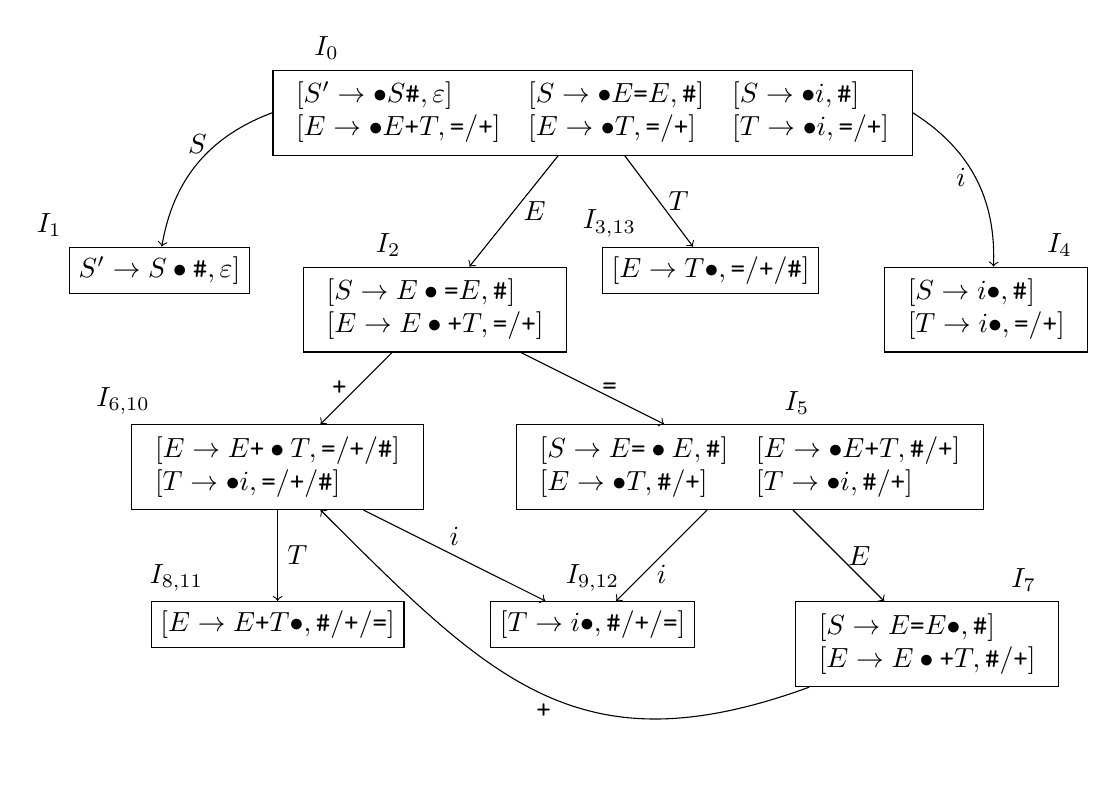
\begin{tikzpicture}
\node[draw,rectangle,label={170:$I_0$}] (I0) at (0,0) {$\begin{array}{lll}
  [S'\rightarrow\bullet S\eof,\varepsilon] & [S\rightarrow\bullet E\tteq E,\eof] & [S\rightarrow\bullet i,\eof]\\\relax
  [E\rightarrow\bullet E\ttpl T,\tteq/\ttpl] & [E\rightarrow\bullet T,\tteq/\ttpl] & [T\rightarrow\bullet i,\tteq/\ttpl]
\end{array}$};
\node[draw,rectangle,label={165:$I_1$}] (I1) at (-5.5,-2) {$S'\rightarrow S\bullet\eof,\varepsilon]$};
\node[draw,rectangle,label={120:$I_2$}] (I2) at (-2,-2.5) {$\begin{array}{l}
  [S\rightarrow E\bullet\tteq E,\eof] \\\relax
  [E\rightarrow E\bullet\ttpl T,\tteq/\ttpl]
\end{array}$};
\node[draw,rectangle,label={160:$I_{3,13}$}] (I3_13) at (1.5,-2) {$[E\rightarrow T\bullet,\tteq/\ttpl/\eof]$};
\node[draw,rectangle,label={40:$I_4$}] (I4) at (5,-2.5) {$\begin{array}{l}
  [S\rightarrow i\bullet,\eof]\\\relax
  [T\rightarrow i\bullet,\tteq/\ttpl]\end{array}$};
\node[draw,rectangle,label={160:$I_{6,10}$}] (I6_10) at (-4,-4.5) {$\begin{array}{l}
  [E\rightarrow E\ttpl\bullet T,\tteq/\ttpl/\eof]\\\relax
  [T\rightarrow\bullet i,\tteq/\ttpl/\eof]\end{array}$};
\node[draw,rectangle,label={60:$I_5$}] (I5) at (2,-4.5) {$\begin{array}{ll}
  [S\rightarrow E\tteq\bullet E,\eof] & [E\rightarrow\bullet E\ttpl T,\eof/\ttpl]\\\relax
  [E\rightarrow\bullet T,\eof/\ttpl] & [T\rightarrow\bullet i,\eof/\ttpl]
\end{array}$};
\node[draw,rectangle,label={160:$I_{8,11}$}] (I8_11) at (-4,-6.5) {$[E\rightarrow E\ttpl T\bullet,\eof/\ttpl/\tteq]$};
\node[draw,rectangle,label={90:$I_{9,12}$}] (I9_12) at (0,-6.5) {$[T\rightarrow i\bullet,\eof/\ttpl/\tteq]$};
\node[draw,rectangle,label={30:$I_7$}] (I7) at (4.25,-6.75) {$\begin{array}{l}
  [S\rightarrow E\tteq E\bullet,\eof]\\\relax
  [E\rightarrow E\bullet\ttpl T,\eof/\ttpl]\end{array}$};

\path[->] (I0.west) [bend right] edge [above] node {$S$} (I1);
\path[->] (I0) edge [right] node {$E$} (I2);
\path[->] (I0) edge [right] node {$T$} (I3_13);
\path[->] (I0.east) [bend left] edge [left] node {$i$} (I4);
\path[->] (I2)edge [left] node {$\ttpl$} (I6_10);
\path[->] (I2) edge [right] node {$\tteq$} (I5);
\path[->] (I6_10) edge [right] node {$T$} (I8_11);
\path[->] (I6_10) edge [above] node {$i$} (I9_12);
\path[->] (I5) edge [below] node {$i$} (I9_12);
\path[->] (I5) edge [right] node {$E$} (I7);
\path[->] (I7) [out=200,in=315,looseness=1.2] edge [below] node {$\ttpl$} (I6_10);
\end{tikzpicture}
\end{document}